\documentclass[a4paper,11pt,titlepage]{jsarticle}

% 画像
\usepackage[dvipdfmx]{graphicx}
\usepackage{here}



\begin{document}
\section{実験結果}
測定日時: 2021年12月29日

bufferであるかないかで大きな差が生じたので、bufferを使わない
実験結果を含めたグラフと、bufferを使いサイズを調整したグラフの二つを
作成した。

作成したグラフは以下の通り(図\ref{1},\ref{2})となった。

\begin{figure}[H]
    \centering
    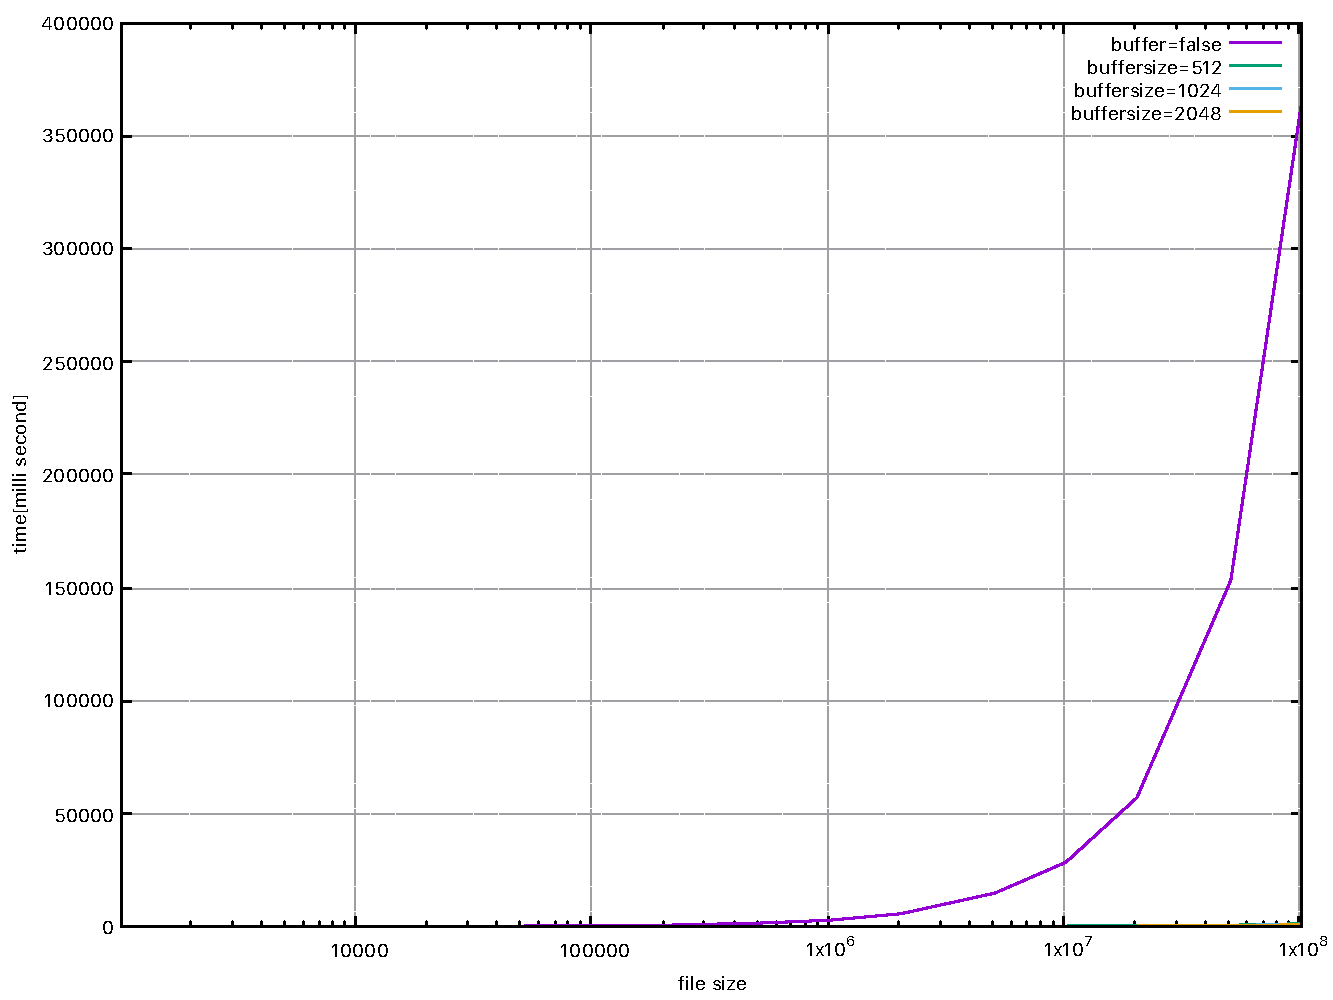
\includegraphics[width=100mm]{./results/buff_and_not.pdf}
    \caption{bufferなしを含む実験結果}
    \label{1}
\end{figure}

\begin{figure}[H]
    \centering
    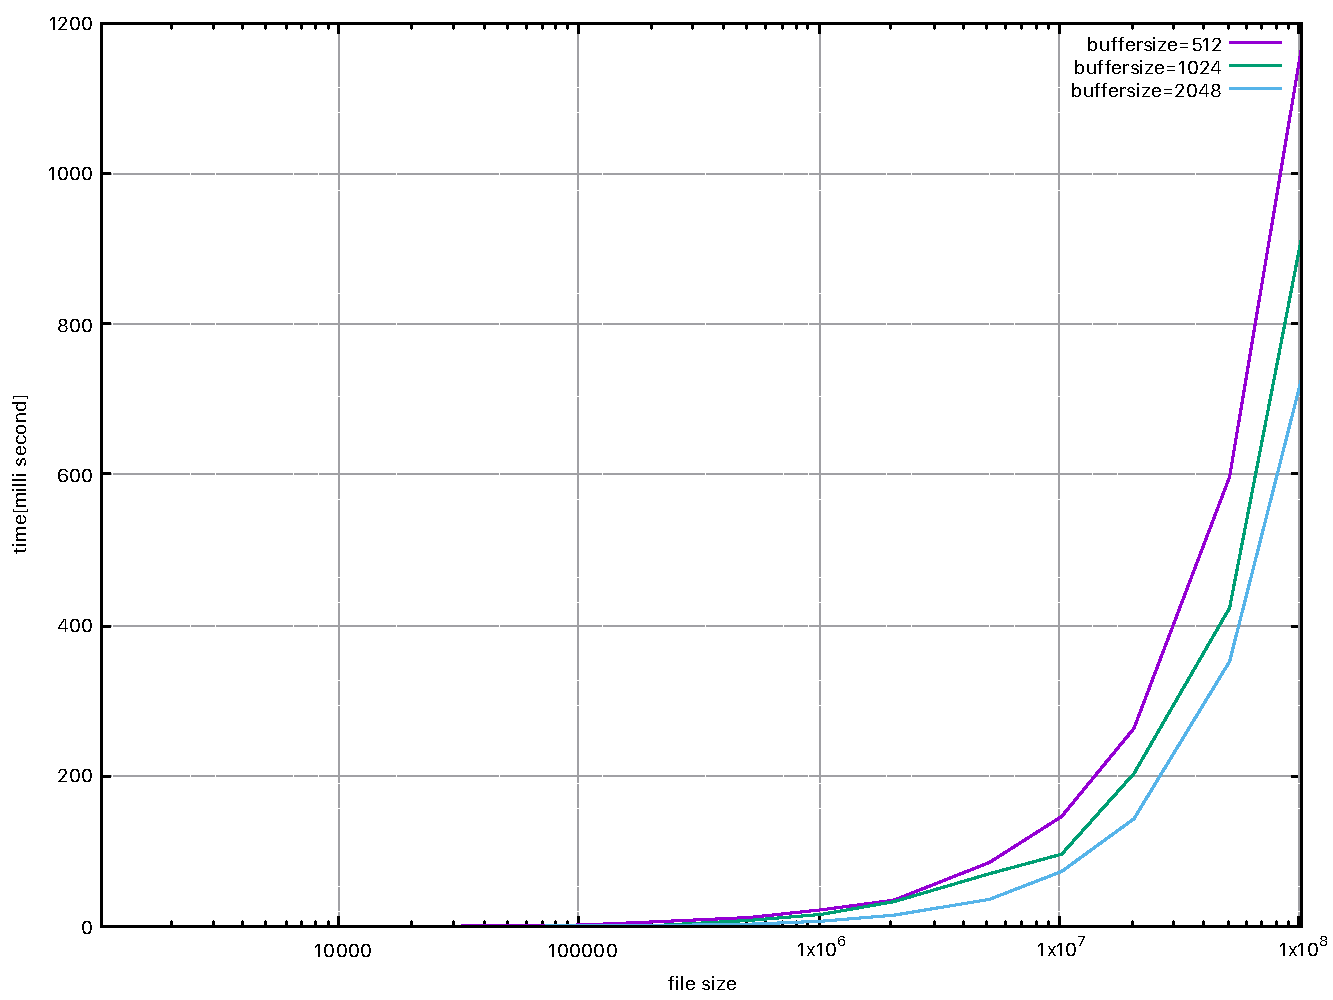
\includegraphics[width=100mm]{./results/buff_only.pdf}
    \caption{bufferサイズを変えて比較した実験結果}
    \label{2}
\end{figure}

\section{考察}
結果から、bufferサイズが大きいほど少ない時間で処理をすることができるとわかる。

したがって、ファイル書き込みの際はbufferサイズを大きくすればかかる時間を
短縮することができると考えられる。

しかし、ファイルサイズが小さい場合はbufferサイズを大きくしても大きな差が見れない
場合があるので、ファイルサイズの大きさによってbufferサイズを適切に設定する
必要がある。

\end{document}